

\newcommand{\argmax}{\operatornamewithlimits{arg\ max}}
\newtheorem{theorem}{Theorem}[section]
\newtheorem{lemma}[theorem]{Lemma}
\newtheorem{property}[theorem]{Property}

\chapter{Industrial Wireless Technology And Applications}\label{chapter:reswk}

% Some very useful LaTeX packages include:
% (uncomment the ones you want to load)
	
\chapterintro*

The use of wireless technologies within factories demands a comprehensive understanding of the problems and potential solutions associated with the rigors of the manufacturing environment. A clearly defined problem space would significantly ease the selection and deployment of appropriate wireless solutions to connected factory systems.  A mapping of potential technologies to classes of use cases within the problem space will be useful to factory operators, system integrators, and wireless systems manufacturers.  Identification of use cases, not addressed by existing technologies, may be used to spur targeted innovation where reliability, resilience, latency, and scalability are joint concerns. Motivated by the industry need for independent practical guidelines and solutions to difficult wireless control problems, this chapter provides a classification of the problem categories where networking technologies may be deployed. It then maps specific technologies that may serve as interim or terminal solutions for those use cases identified within the problem space taxonomy. This chapter is intended to provide a detailed exposition of the requirements directed towards industrial wireless.  It draws on various sources of requirements captured by academic literature, industry organizations, and standards institutes.  The work therefore presents a picture of the requirements landscape at the beginning of this research.  Further work in this area is found in~\cite{Montgomery2019} and~\cite{Raptis2019}.

	\section{Introduction} \label{sec:intro}
%    \subsection{Purpose}
    Industrial wireless is a key enabling technology for the \glspl{iiot}.  The \gls{iiot} promises lower costs of deployment, increased mobility of factory assets, massive interconnectivity, improved situational awareness, increased efficiency of the operation, and improved operations analytics.  IIoT and advanced manufacturing technology seek to improve competitiveness, productivity, and responsiveness to customer needs. However, it is often stated that where wireless is deployed, factory enhancements fail to meet expectations typically in areas of reliability, resilience, and scalability. Moreover, transmission security is often cited as an area of concern. Risk averse organizations will establish policies that preclude wireless to be deployed for specific types of applications such as feedback control or safety. Yet, factory operators are increasingly demanding that wireless be deployed for critical and sometimes conceivably dangerous applications.  For this reason, \gls{nist} is developing best practice guidelines to help factory operators select appropriate wireless systems for their particular use case and then deploy that solution effectively.  Such a mission requires participation by factory operators, system integrators, and device manufacturers. A comprehensive taxonomy of the existing problem space within industry and a survey of existing and missing technologies are necessary to the success of such a mission. This chapter provides our classification of industrial wireless cases and links current technologies to those use cases if applicable. 
    
%    \subsection{Related Work}
%    %Mohamed will provide.  High level mentions and limitation.  Stop.
%The use of industrial wireless networks has been studied in many works in the literature. However, no comprehensive survey of the whole problem space of industrial communications has been performed.
%
%In \cite{6248648}, the authors have introduced a comparison between the commercial and industrial communications networks where an industrial network has been divided to five different levels. These levels include field equipment, controller level, application, supervisory, and external networks. The differences in requirements between different levels are discussed. Moreover, three types of information are considered which are control, diagnostic, and safety information as described in \cite{4118467}. However all these levels of industrial networks are mentioned in \cite{6248648}, the article focuses only on the manufacturing and instrumentation communications and does not consider other types of communications networks that exist in industrial environments. Also, in \cite{What}, three levels of communications are considered which are device, control, and information levels. Moreover, the current wired industrial technologies for these levels are discussed briefly.
%
%More works focused on the communications at the field devices level where sensing and control information is transfered. In \cite{7005074},  the communication between field devices has been studied where the requirements for a large number of nodes may not be achieved. The use of fieldbus solutions limit the scalability and resilience and hence industrial Ethernet capabilities are introduced in this article. Moreover, in \cite{Connectivity}, the communication for monitoring and control operations is discussed. A comparison between fieldbus technologies, industrial Ethernet, and wireless solutions is performed. The author has discussed the use of Wi-Fi, Bluetooth, ZigBee, and WirelessHART technologies in industrial applications. Similarly, the authors of \cite{6490786} considered the industrial communications networks requirements in process automation specifically at field devices level. Finally, in \cite{GE_Professional}, many case-studies are discussed for communication networks in industrial scenarios. Moreover, the design steps for these solutions are briefly discussed.

%    \subsection{Paper Organization}
%    The rest of the paper is organized as follows. The problem space for employing wireless networks is presented in Section II. Then, the technical considerations while designing industrial wireless networks are discussed briefly in Section III.  In Section IV, a mapping between the problem space and the current technology space is provided. Finally in Section V, future directions and conclusions are presented.
    
    \section{Problem Space}
    
    \subsection{Introduction and Success Considerations}
    Implementing a factory enhancement program requires economic and technical planning, and justification.  Wireless technologies by themselves are interesting and can provide value; however, it is incumbent upon plant leadership to fully assess the potential risks and benefits of the enhancement before proceeding with deployment. Wireless technologies are often deployed as a means to monitor or control factory process. They have the potential to unlock improved observability and control. By understanding the problem space and the risks and benefits of potential wireless solutions, factory operators can assess if the rewards outweigh the risks.  In navigating the risk/reward question, it is asserted that any wireless program must address one or more of the following success criteria before embarking on an enhancement involving wireless communications.  These criteria are defined as follows:
    
	\paragraph{Reliability} Wireless systems can be deployed to add redundancy or replace faulty wired solutions with a more reliable wireless solution for particularly harsh industrial environments where temperature, pressure, vibration, radiation, and chemistry may make wired communication unreliable.
	\paragraph{Safety} Wireless systems may be used to detect or prevent injury to humans.  They may be used as backup to wired systems or serve as the primary communication system.
	\paragraph{Production Cost} Wireless systems can increase observability and the resulting data may be used for precise optimization of the factory operations, machine scheduling, and maintenance.
	\paragraph{Quality} Various measurements are possible to improve quality of the factory output. Using wireless solutions may make deployment of sensors and inspection equipment more practical. 
	\paragraph{Environment} Wireless sensors and control mechanisms may be used to detect toxic conditions and prevent environmental accidents from occurring.  Wireless actuation devices may serve to improve reliability and address environmental mitigation control. 
	\paragraph{Regulations} In some scenarios, government regulations may require specific sensor instrumentation to be deployed for certain scenarios.  Wireless solutions could make regulatory compliance practical or cost effective in some cases.
      
    \subsection{Use Cases}
    
    Once a plant upgrade enhancement program is initiated, and some type of wireless technology is anticipated, the first step in realizing the program is defining and understanding the problem space where wireless technologies will be used. To support this assessment, a taxonomy of industrial use cases to which wireless communication may be employed is given.  The industrial wireless landscape is diverse, and a classification of those technologies can be helpful in mapping particular technologies to an application.  Our classification is shown in Fig.~\ref{fig:problemspace} and includes instrumentation, safety, and back-haul connectivity, among others. Each class of the problem space is explained in the following subsections.  

\begin{figure}[t]
\centering
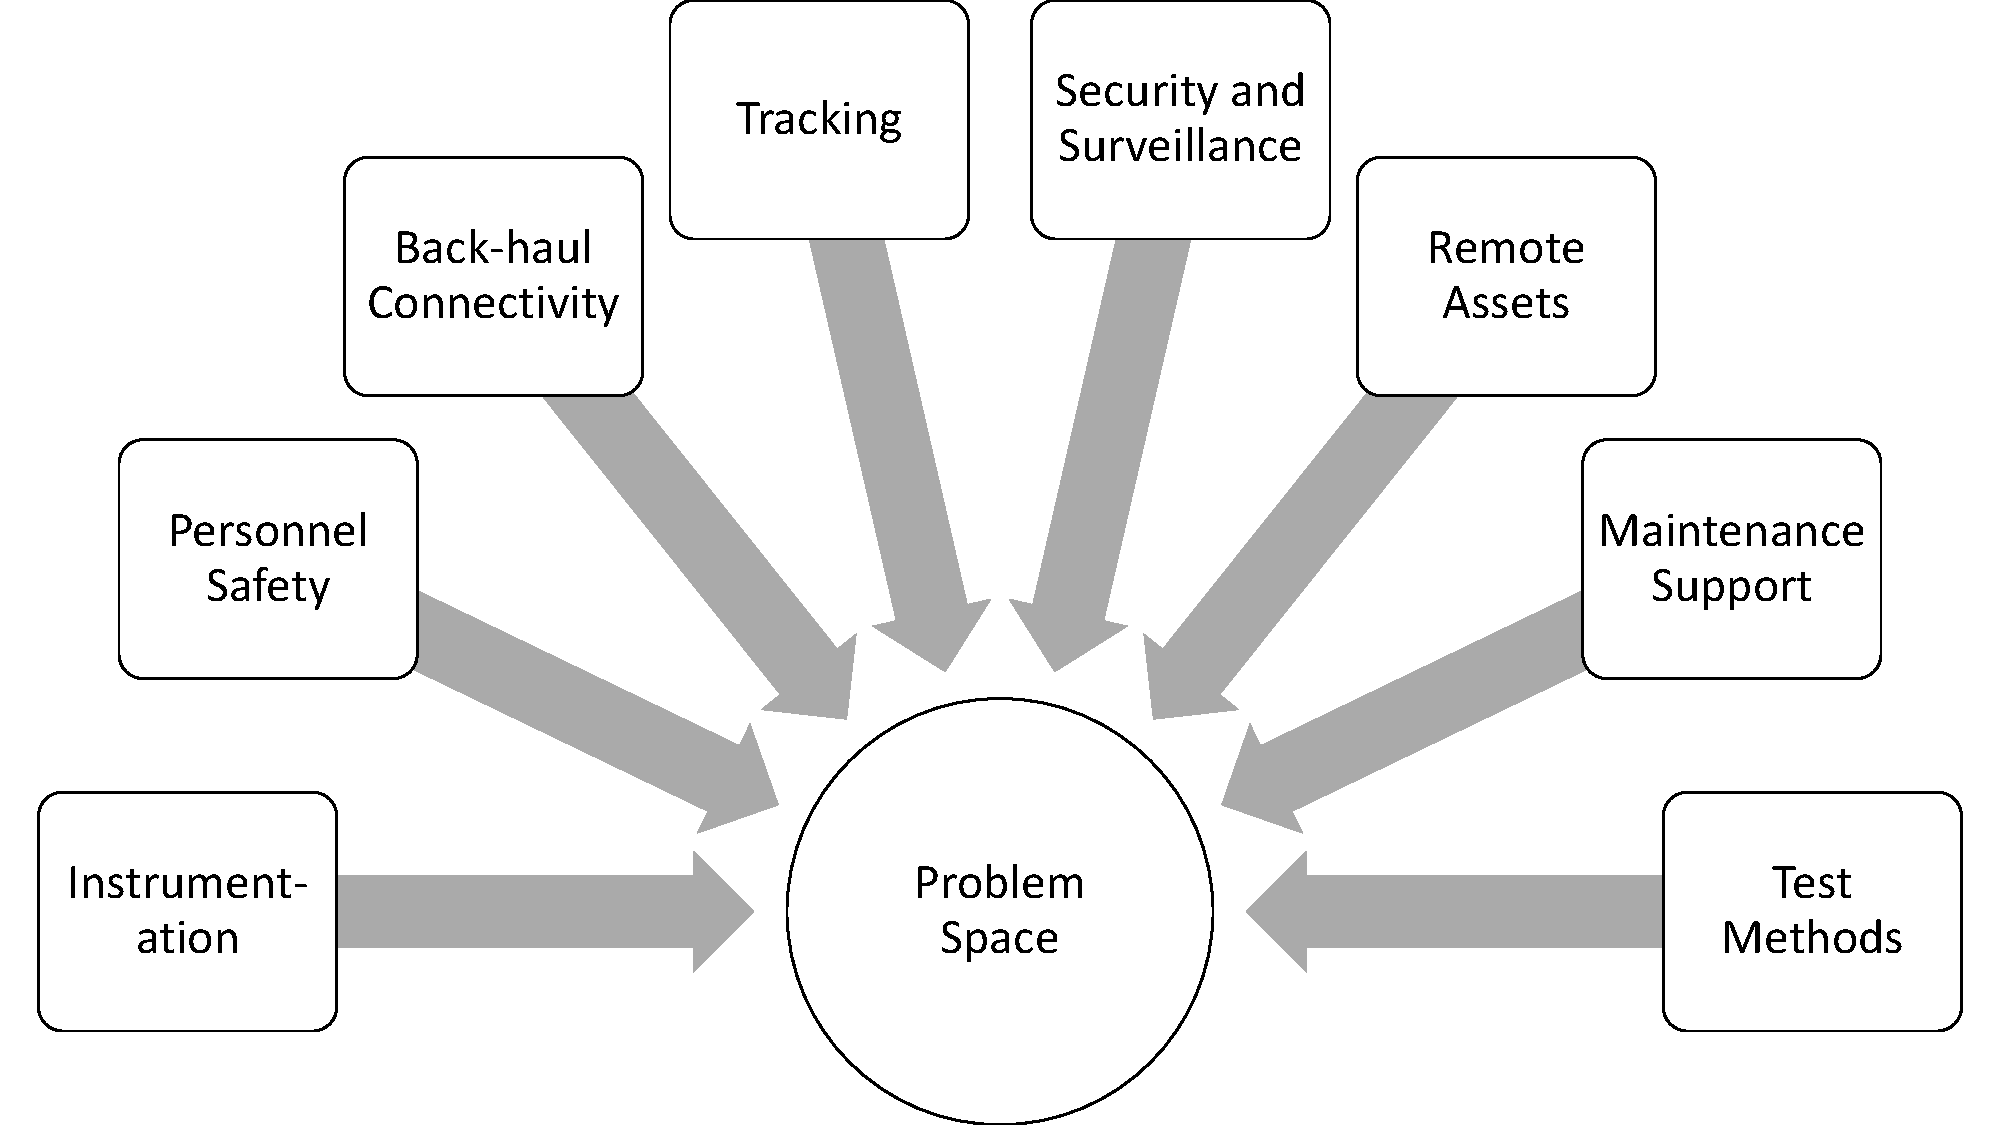
\includegraphics[width=\columnwidth]{./chapter-reswk/figs/probsp}
\caption{Industrial wireless technologies are applicable across most aspects of the industrial automation problem space.}
\label{fig:problemspace}
\end{figure}   

    \subsubsection{Manufacturing Instrumentation}  
    Manufacturing instrumentation includes devices commonly known as sensors and actuators.  Sensors transmit measured variables from the physical process.  Actuators receive manipulation variables from a controller and apply changes to the physical process. This class of application demands typically a very low latency and high reliability communication channel.  
    
    \subsubsection{Personnel Safety}  
    Industrial settings can be hazardous to both humans and machines.  For humans, conditions may arise that pose a substantial risk for injury or death.  For machines, conditions may develop that cause substantial damage requiring extensive repair or replacement.  Prevention of industrial accidents is therefore of paramount importance within factories~\cite{Smith201788}.  Slips, trips, and falls on the same level are commonly cited as lead causes of injury~\cite{Chang2016}. Falls from higher levels are of great concern to the aerospace industry~\cite{Candell2017IWW} as inspection teams must work on elevated levels where falls prove fatal.  Within the oil and gas industry, safety concerns include air toxicity and combustibility in both open and confined spaces where reliable monitoring and reporting save lives. Wireless gas leak detection and leak localization provide important and effective safety enhancements to such systems~\cite{Chraim2016}.  Within smart manufacturing systems where humans and robots work closely and even within traditional robot environments, safety systems provide an added layer of protection to prevent human injury~\cite{Huber:2017:DHI:3029798.3038346}, \cite{Zanchettin2016}.  Within these human-robot environments, it is clear that reliable, low-latency communication is an important aspect of safety implementation, and, as mobility of robots within the factory increases, reliable low-latency wireless networks will become increasingly important to safety implementation.
    
    \subsubsection{Back-haul Connectivity}  The back-haul is generally defined as the network that connects a lower level network to a higher level network \cite{7456186}. Back-haul connectivity is usually characterized by large amounts of transfered data. In industrial environments, various types of back-haul scenarios are needed to be deployed for the operation of industrial communication networks. One can divide the back-haul problem space into three partitions which are i) nearby or indoor back-hauls, ii) distant back-hauls, and iii) geographically remote back-hauls. This categorization is based on the distance over which data is transfered.
    
First, the indoor back-haul networks are used in factory floors or process plants for data transfer between the control level networks to data centers, and higher level application layer networks. Second, the distant back-hauls are used for information transfer between various buildings in a plant where the two ends  may have a \gls{los} or need a \gls{nlos} technology \cite{PS-backhaul}. Finally, the geographically remote back-hauls are used for information transfer between sites in different cities or even countries such as data transfer to headquarters. Various technologies which are currently used for back-haul networks are discussed in \cite{PS-backhaul}.   
    
    \subsubsection{Tracking}
Tracking in industrial environments is employed to follow the states of inventory, personnel, and tools which help in process control and factory management \cite{PS_tracking2}. The focus of this class of the problem space is the set of transmissions related to the tracking process itself and not the recovered data transmissions back to higher levels. Wireless tracking systems are subdivided into the following divisions based on various requirements: i) materials tracking, ii) personnel tracking, iii) tools tracking, iv) inventory management, v) localization, and vi) identification. 

Materials, personnel, and tools tracking is focused on following the state and the location of the tracked item. The selection of the used technology will depend on the tracked item characteristics including its speed, required accuracy level, and scalability. Inventory management includes the decisions related to the change of inventory status over time. Identification and localization are required for the determination of the position and identity of a person or an item at a specific situation or time. It can be important in safety and security related applications. 

The characteristics and applications of various tracking, localization, and identification technologies are discussed in~\cite{PS_tracking2}. These technologies include the use of specific wireless communications technologies like \gls{gps}, and \gls{rfid} or deploying the general-purpose technologies like \gls{wifi}, Bluetooth, and the cellular-based technologies. Moreover, examples of the existing products for assets tracking and their performance are compared in \cite{PS-tracking1}.  


    
    \subsubsection{Security and Surveillance}  
    Industrial installations require protection of the physical grounds, the operation, and the data produced from the installation.  This protection requires surveillance of the property and implementation of network security controls. Guidance on selecting which controls are applicable to a specific risk level may be found in~\cite{Stouffer2015}. Assessment of the security robustness of specific wireless technologies is outside the scope of this work; however, the implementation of physical security controls such as personnel authorization and grounds protection requires transmission of varying amounts of data.  Transmission of such data includes voice traffic, video, and status information.  In some installations, security and surveillance transmissions will coexist with factory instrumentation.  This is sometimes the case with \gls{ieee} 802.11 mesh networks carrying voice, video, and instrumentation traffic.  
    
    \subsubsection{Remote Assets} 
Remote monitoring and control extend the range of the management to remote sites, especially in the process industry. Industrial remote communications provide access to widely distributed assets such as wellhead and pipeline monitoring \cite{PS-remote2}. The main goals of employing remote monitoring and control are minimizing labor cost, improved operations of remote sites, and prevention of  unplanned failures \cite{PS-remote1}. 

The use of wireless networks in remote monitoring and control reduces the installation and maintenance cost significantly. However, the main challenge for industrial wireless remote monitoring and control is security and hence encryption and authentication protocols are deployed. Examples of remote assets communications are discussed in \cite{PS-remote2}.      
    
    \subsubsection{Maintenance Support}  
    Factories require maintenance teams to keep machinery operating efficiently.  Machines may be instrumented with sensors that measure machine health data such as vibration levels or current calibration values.  Using this information, machines can be scheduled for maintenance prior to failure thereby allowing the factory to operate without unexpected interruption.  Maintenance of the factory may also include automation of the building and infrastructure for climate control.  \Gls{hvac} systems can be automated such that the ambient conditions are controlled.  Augmented reality is an emerging technology that promises to bring knowledge to the factory floor allowing maintenance personnel to gain access to information during uncertain situations~\cite{Paelke2014}.  Augmented reality is a high-bandwidth application that requires high-reliability, high-throughput wireless connectivity within the factory.
    
    \subsubsection{Test Methods}  
Industrial control systems are often intolerant of communication faults and network latency, and often require very high transmission reliability~\cite{Zhang2013}. Depending on the purpose of the wireless network (monitoring, supervisory control, feedback control, or safety monitoring), understanding the system performance of the network may be critical. For feedback control and safety monitoring systems, understanding the performance of the network from the perspective of the industrial controller or safety alarm system is essential. Factory operators, system integrators, and control systems designers are rarely experts in wireless communications systems.  Considerations such as electromagnetic propagation, antenna efficiency, path loss exponents, packet error rates, and medium access are often foreign concepts to factory engineers.  If factory engineers are expert in wireless theory and design practice, the information that they need to make educated decisions are usually unavailable.  When available, link quality metrics such as packet loss ratios are informative but can be difficult to understand with complex mesh architectures and routing algorithms.

Moreover, it is generally difficult to measure these quantities for operational networks. The control system designer will only need to know the statistical distribution of latency and reliability of information through the network to design a controller that is robust. Therefore, practical methods for characterizing the performance of the wireless network that do not require an in-depth understanding of wireless communications or electromagnetic wave propagation are needed.

\begin{emphbox}
	A clear need for accessible test methods exists in the wireless \glspl{cps} space in which the tester need not be an expert in wireless communications or radio wave propagation.
\end{emphbox}

    
    \section{Technical Considerations}

    \subsection{Radio Frequency Environment}
   Using wireless communications in industrial environments requires the knowledge of the \gls{rf} environment characteristics and their behavior under the added wireless networks. The first step is obtaining and modeling field data in industrial environments. In \cite{Candell2017}, the RF environments of multiple examples of industrial scenarios were studied where models and characterization parameters have been derived. Moreover, theoretical models are proposed to model the RF channel such as the IEEE802.15.4a model including its channel impulse response \cite{A.F.Molisch2004}. In characterizing the RF environments, various parameters should be included, such as the multi-path, the interference sources, the mobility, and shadowing effects. Moreover, the operating frequency band can play an important role based on the required performance and the nature of RF activity in a certain environment.
   
%   Rick: reference NIST-TN-1951 
%    Are things changing in the environment?
%    Multi-path (IEEE 802.15.4a report)
%    What are the interference sources
%    What are the distances between wireless nodes
%    If mobile links or changing environment: shadowing effects
%    Does a mobility model apply to the scene
%    Is it indoor/outdoor?
%    RFBand selection: 900, 2400, 5000
%    mmwave~\cite{Cheffena7565190}
    
    \subsection{Device Characteristics}  
Another important aspect while deploying wireless networks in industrial environments is the used devices characteristics. Typically, the harsh industrial environments in many applications require higher ratings of the used devices. The considered device characteristics include size, weight, power, cost, safety, and ingress protection ratings. Based on the application requirements and the physical environments, these device requirements are determined.



%Device consideration include size, weight, power, cost, environmental, and safety. When considering the size of the devices
%    IP64-66 rating (Ingress Protection) Rating
%    intrinsic safety rating for combustible environments
%    shock, vibration, heat, humidity, etc.
    
    \subsection{Network Characteristics}
    
Table~\ref{tbl:techreqs} lists requirements typically expected of a network based on its intended purpose and problem domain.  Industrial networks will have three basic characteristics: reliability, latency, and scale.  These characteristics are described in the following subsections.  The numbers listed in the table are based on existing applications.  It is difficult to provide a standard metric for all use cases as each will impose different requirements on the network.  In some cases, the control algorithm can be designed to adapt to information loss and delay, thereby improving the performance of the physical system.

	\subsubsection{Latency} Latency is a measure of the delay that information takes to arrive at its destination.  Latency, $l$, is defined as the measured delay from the time of an event to the time in which knowledge of that event is made available to an application. Using the \gls{osi} model as a guide, latency would be measured at the application layer.  In a packaging system, an example of measured latency would be the time between a proximity event and the time knowledge of that event is received by a \gls{plc}. 
    
    \subsubsection{Reliability} Reliability is a measure of the likelihood of data loss within the industrial network.  Reliability, $r$, is defined as the probability that a block of transmitted data is delayed long enough to become obsolete or lost due to noise.  Similar to latency, reliability is measured at the application layer thereby ignoring technology-specific issues such as data segmentation and retries similar to the approach taken in the developing \gls{5g} cellular networks for machine-to-machine communications~\cite{Holfeld2016}.
    
    \subsubsection{Scale} Scale is a measure of the number of devices that may be deployed within a network without sacrificing reliability or latency. The network size will often dictate the maximum bandwidth allotted to any one node.  The larger the network, the less bandwidth is alloted for transmissions between nodes.  The complexity of a fully interconnect mesh will theoretically exhibit factorial growth in network interconnections.  In practice, \glspl{snr} between nodes, programming within the governing network controller, and provisioned constraints will limit the number of interconnections.  Most \gls{wsn} specifications such as WirelessHART, ISA100.11a, and Zigbee provide support for large scale deployments; however, in such deployments, the network infrastructure must support the throughput load of the network and the scan rate requirements of the factory application~\cite{Wang7448365}.  The ISA100.11a standard provides support for distributed access points, prescribed routing, and a partitioned architecture to allow for large-scale deployments.

% Requirements table
\begin{table}[!t]
	\centering
	\caption{Industrial control latency, error rate, and scalability considerations for wireless deployments as presented in~\cite{CandellRW2017} show important and competing considerations of industrial wireless deployments.  Other considerations not shown include battery life, update rate, and security, among others. }
	\label{tbl:techreqs}
	% Table generated by Excel2LaTeX from sheet 'reqs'
\begin{tabular}{llll}
 &
  Latency, $l$ \si{ms} &
  Pr. Loss, $r$ &
  Scale, $s$
  \\
\midrule
Monitoring &
  $l<1000$ &
  $r<10^{-5}$ &
  $s<10,000$
  \\
\midrule
Supervisory Control &
   &
   &
  
  \\
   Flow-based &
  $l<1000$ &
  $r<10^{-6}$ &
  $s<30$
  \\
   Job-based &
  $l<100$ &
  $r<10^{-7}$ &
  $s<10$
  \\
\midrule
Feedback Control &
   &
   &
  
  \\
   Flow-based &
  $l<1000$ &
  $r<10^{-6}$ &
  $s<100$
  \\
   Job-based &
  $l<10$ &
  $r<10^{-7}$ &
  $s<10$
  \\
\midrule
Safety &
  $l<10$ &
  $r<10^{-7}$ &
  $s<10$
  \\
\bottomrule
\end{tabular}%

\end{table}%

    \subsubsection{Interoperability}
    In a factory application, easy integration of devices is essential to the flow of data through a network. While many wireless standards exist, making physical layer integration of devices within the wireless domain easier, most industrial networks fail to address the application layer well.  WirelessHART describes an application layer interface, while ISA100.11a provides the constructs for such an interface.  ZigBee and \gls{wifi} provide neither the interface nor the constructs for an application layer protocol. On the back-haul side of wireless networks which usually begins at a wireless gateway and ends at an automation server, many protocols such as \gls{opc} and Modbus make integration easier; however, again, they fail to specify the interface but instead provide the constructs.  The authors assert that a standardization of the automation interface (gateway to automation server) is needed to provide such interoperability. 
    
    \subsubsection{Security}
    Prescribing security controls within an automation system requires understanding of the risk of not implementing these controls and the impacts of them on the physical process. Work is being undertaken to measure the impacts of cyber-security controls on the physical process as explained in~\cite{candell2015industrial} and~\cite{candell2015measuring}. In addition, the work is being undertaken to assess the impacts of stealthy attacks as described in~\cite{urbina2016limiting}. \gls{nist} Special Publication 800-82 and \gls{iec}-62443 provide best practice guidelines for the implementation of a cyber-security program in an automation system.
    
    \section{Wireless Technology Applicability}
    Many existing wireless technologies could be applied to the use cases in Section II.  Others may be applicable with limitations, and others are not applicable entirely. Table~\ref{tbl:techmap} captures mapping of technologies to applicable use cases.  This table represents assertions by the authors of applicability of wireless technologies to industrial control systems problem domains based on industry practice and original intent of the technology.  The authors assert that the problem domains and wireless technologies included within this table represent the majority  of problems found within industry and the existing technologies that may be applied.  Technologies were evaluated based on original design intent, latency, reliability, energy, and practicality.  Modifications may be made to the listed technologies resulting in applicability to a specified problem; however, possible modifications were not considered.  \Gls{vlbr} \glspl{wan} are assumed to have an infrastructure-based  topology and support a bit rate of under 600bps. 
    
% Table generated by Excel2LaTeX from sheet 'mapping'
\begin{table*}[htbp]
	\setlength{\tabcolsep}{1.4pt}
  	\centering
  	\caption{Applicability of wireless technologies from~\cite{CandellRW2017}.  Presented are recommendations of direct applicability of various technologies to the industrial user problem space with little to no modification. }
  	\label{tbl:techmap}%
  	\begin{adjustbox}{width=\textwidth}
	% Table generated by Excel2LaTeX from sheet 'mapping'
\begin{tabular}{l|l|ccccc|cccccc|cccc|cccc|ccccc|cccccc|ccc|ccc}
\multicolumn{1}{r}{} &
  \multicolumn{1}{r}{} &
  \begin{sideways}Process Monitoring\end{sideways} &
  \begin{sideways}Supervisory Control\end{sideways} &
  \begin{sideways}Feedback Control\end{sideways} &
  \begin{sideways}Alarm Conditions\end{sideways} &
  \multicolumn{1}{c}{\begin{sideways}In-situ Inspection\end{sideways}} &
  \begin{sideways}Factory Monitoring\end{sideways} &
  \begin{sideways}Assembly: Sensing\end{sideways} &
  \begin{sideways}Assembly: Actuation\end{sideways} &
  \begin{sideways}Robots: Supervision\end{sideways} &
  \begin{sideways}Robots: Feedback Control\end{sideways} &
  \multicolumn{1}{c}{\begin{sideways}Quality Inspection\end{sideways}} &
  \begin{sideways}Fall Prevention\end{sideways} &
  \begin{sideways}Confined Spaces\end{sideways} &
  \begin{sideways}Critical Event Detection\end{sideways} &
  \multicolumn{1}{c}{\begin{sideways}Human-Machine Colocation\end{sideways}} &
  \begin{sideways}Nearby or Indoor\end{sideways} &
  \begin{sideways}Distant: LOS\end{sideways} &
  \begin{sideways}Distant: BLOS\end{sideways} &
  \multicolumn{1}{c}{\begin{sideways}Geographically Remote\end{sideways}} &
  \begin{sideways}Indoor Machine Localization\end{sideways} &
  \begin{sideways}Materials in Storage\end{sideways} &
  \begin{sideways}Materials in Production\end{sideways} &
  \begin{sideways}Tools\end{sideways} &
  \multicolumn{1}{c}{\begin{sideways}Personnel\end{sideways}} &
  \begin{sideways}Voice and Video Communication\end{sideways} &
  \begin{sideways}Video Survellience\end{sideways} &
  \begin{sideways}Drone-based Surveillance\end{sideways} &
  \begin{sideways}Grounds Control\end{sideways} &
  \begin{sideways}Spectrum Monitoring Data\end{sideways} &
  \multicolumn{1}{c}{\begin{sideways}Personnel Authorization\end{sideways}} &
  \begin{sideways}Well-head Monitoring\end{sideways} &
  \begin{sideways}Pipeline Monitoring\end{sideways} &
  \multicolumn{1}{c}{\begin{sideways}Tank Level Monitoring\end{sideways}} &
  \begin{sideways}Machine Health Monitoring\end{sideways} &
  \begin{sideways}Building Automation\end{sideways} &
  \begin{sideways}Augmented Reality\end{sideways}
  \\
\multicolumn{1}{r}{} &
  \multicolumn{1}{r}{} &
  \multicolumn{5}{c|}{Flow-based} &
  \multicolumn{6}{c|}{Job-based} &
  \multicolumn{4}{c|}{Safety} &
  \multicolumn{4}{c|}{Back-haul} &
  \multicolumn{5}{c|}{Tracking} &
  \multicolumn{6}{c|}{Security} &
  \multicolumn{3}{c|}{Remote} &
  \multicolumn{3}{c}{Maint.}
  \\
\midrule
\multirow{2}[2]{*}{Home/Office} &
  IEEE 802.11 &
  \CIRCLE &
  \CIRCLE &
  \LEFTcircle &
  \LEFTcircle &
  - &
  \CIRCLE &
  \LEFTcircle &
  \LEFTcircle &
  \LEFTcircle &
  \LEFTcircle &
  \LEFTcircle &
  \fullmoon &
  \fullmoon &
  \LEFTcircle &
  \fullmoon &
  \CIRCLE &
  \CIRCLE &
  \CIRCLE &
  - &
  \LEFTcircle &
  \lightning &
  \lightning &
  \lightning &
  \multicolumn{1}{c}{\lightning} &
  \CIRCLE &
  \CIRCLE &
  \CIRCLE &
  \CIRCLE &
  \CIRCLE &
  \CIRCLE &
  \LEFTcircle &
  \fullmoon &
  \LEFTcircle &
  \LEFTcircle &
  \CIRCLE &
  \CIRCLE
  \\
 &
  IEEE 802.15.1 &
  \fullmoon &
  \fullmoon &
  \fullmoon &
  \fullmoon &
  \fullmoon &
  \fullmoon &
  \LEFTcircle &
  \LEFTcircle &
  \LEFTcircle &
  \fullmoon &
  \CIRCLE &
  \fullmoon &
  \LEFTcircle &
  \fullmoon &
  \fullmoon &
  \fullmoon &
  \fullmoon &
  \fullmoon &
  \fullmoon &
  \fullmoon &
  \fullmoon &
  \lightning &
  \CIRCLE &
  \LEFTcircle &
  \DOWNarrow &
  \DOWNarrow &
  \DOWNarrow &
  \fullmoon &
  \fullmoon &
  \LEFTcircle &
  \fullmoon &
  \fullmoon &
  \fullmoon &
  \LEFTcircle &
  \fullmoon &
  \DOWNarrow
  \\
\midrule
\multirow{4}[2]{*}{Industrial} &
  IEEE 802.15.4 TDMA &
  \CIRCLE &
  \CIRCLE &
  \LEFTcircle &
  \LEFTcircle &
  - &
  \CIRCLE &
  \clock &
  \clock &
  \clock &
  \clock &
  \LEFTcircle &
  \clock &
  \LEFTcircle &
  \LEFTcircle &
  \fullmoon &
  \DOWNarrow &
  \DOWNarrow &
  \DOWNarrow &
  \DOWNarrow &
  \LEFTcircle &
  \lightning &
  \lightning &
  \lightning &
  \LEFTcircle &
  \DOWNarrow &
  \DOWNarrow &
  \DOWNarrow &
  \LEFTcircle &
  \DOWNarrow &
  \fullmoon &
  \CIRCLE &
  \CIRCLE &
  \CIRCLE &
  \CIRCLE &
  \CIRCLE &
  \DOWNarrow
  \\
 &
  IEEE 802.15.4 CSMA &
  \LEFTcircle &
  \LEFTcircle &
  \fullmoon &
  \fullmoon &
  - &
  \CIRCLE &
  \clock &
  \clock &
  \clock &
  \clock &
  \LEFTcircle &
  \clock &
  \LEFTcircle &
  \LEFTcircle &
  \fullmoon &
  \DOWNarrow &
  \DOWNarrow &
  \DOWNarrow &
  \DOWNarrow &
  \LEFTcircle &
  \lightning &
  \lightning &
  \lightning &
  \LEFTcircle &
  \DOWNarrow &
  \DOWNarrow &
  \DOWNarrow &
  \LEFTcircle &
  \fullmoon &
  \fullmoon &
  \LEFTcircle &
  \LEFTcircle &
  \LEFTcircle &
  \CIRCLE &
  \CIRCLE &
  \DOWNarrow
  \\
 &
  IEEE 802.11 TDMA &
  \hexstar &
  \hexstar &
  \hexstar &
  \hexstar &
  - &
  \hexstar &
  \hexstar &
  \hexstar &
  \hexstar &
  \hexstar &
  \hexstar &
  \hexstar &
  \hexstar &
  \hexstar &
  \hexstar &
  - &
  - &
  - &
  - &
  \hexstar &
  - &
  - &
  - &
  - &
  - &
  - &
  - &
  \hexstar &
  - &
  - &
  \hexstar &
  \hexstar &
  \hexstar &
  \hexstar &
  \hexstar &
  -
  \\
 &
  VLBR WAN &
  \CIRCLE &
  \CIRCLE &
  \fullmoon &
  \LEFTcircle &
  - &
  \CIRCLE &
  \clock &
  \clock &
  \clock &
  \clock &
  \clock &
  \clock &
  \fullmoon &
  \fullmoon &
  \fullmoon &
  \DOWNarrow &
  \DOWNarrow &
  \DOWNarrow &
  \DOWNarrow &
  \LEFTcircle &
  \LEFTcircle &
  \LEFTcircle &
  \LEFTcircle &
  \LEFTcircle &
  \DOWNarrow &
  \DOWNarrow &
  \DOWNarrow &
  \clock &
  \fullmoon &
  \fullmoon &
  \fullmoon &
  \fullmoon &
  \fullmoon &
  \LEFTcircle &
  \LEFTcircle &
  \fullmoon
  \\
\midrule
\multirow{3}[2]{*}{Satellite} &
  Geostationary &
  \LEFTcircle &
  \LEFTcircle &
  \fullmoon &
  \fullmoon &
  \fullmoon &
  \fullmoon &
  \fullmoon &
  \fullmoon &
  \fullmoon &
  \fullmoon &
  \fullmoon &
  \fullmoon &
  \fullmoon &
  \fullmoon &
  \fullmoon &
  \fullmoon &
  \fullmoon &
  \fullmoon &
  \LEFTcircle &
  \fullmoon &
  \fullmoon &
  \fullmoon &
  \fullmoon &
  \fullmoon &
  \LEFTcircle &
  \LEFTcircle &
  \fullmoon &
  \LEFTcircle &
  \LEFTcircle &
  \LEFTcircle &
  \LEFTcircle &
  \LEFTcircle &
  \LEFTcircle &
  \fullmoon &
  \fullmoon &
  \LEFTcircle
  \\
 &
  Low-earth Orbit &
  \LEFTcircle &
  \LEFTcircle &
  \fullmoon &
  \fullmoon &
  \fullmoon &
  \fullmoon &
  \fullmoon &
  \fullmoon &
  \fullmoon &
  \fullmoon &
  \fullmoon &
  \fullmoon &
  \fullmoon &
  \fullmoon &
  \fullmoon &
  \fullmoon &
  \fullmoon &
  \LEFTcircle &
  \LEFTcircle &
  \fullmoon &
  \fullmoon &
  \fullmoon &
  \fullmoon &
  \fullmoon &
  \LEFTcircle &
  \LEFTcircle &
  \LEFTcircle &
  \LEFTcircle &
  \LEFTcircle &
  \LEFTcircle &
  \LEFTcircle &
  \LEFTcircle &
  \LEFTcircle &
  \LEFTcircle &
  \fullmoon &
  \LEFTcircle
  \\
 &
  VLBR WAN &
  \LEFTcircle &
  \LEFTcircle &
  \fullmoon &
  \LEFTcircle &
  \fullmoon &
  \clock &
  \clock &
  \clock &
  \clock &
  \clock &
  \clock &
  \clock &
  \fullmoon &
  \fullmoon &
  \fullmoon &
  \DOWNarrow &
  \DOWNarrow &
  \DOWNarrow &
  \DOWNarrow &
  \fullmoon &
  \fullmoon &
  \fullmoon &
  \fullmoon &
  \LEFTcircle &
  \DOWNarrow &
  \DOWNarrow &
  \DOWNarrow &
  \LEFTcircle &
  \fullmoon &
  \fullmoon &
  \fullmoon &
  \fullmoon &
  \fullmoon &
  \LEFTcircle &
  \fullmoon &
  \DOWNarrow
  \\
\midrule
Tracking &
  RFID &
  - &
  - &
  - &
  - &
  - &
  - &
  - &
  - &
  - &
  - &
  - &
  - &
  - &
  - &
  - &
  - &
  - &
  - &
  - &
  \fullmoon &
  \CIRCLE &
  \CIRCLE &
  \CIRCLE &
  \CIRCLE &
  - &
  - &
  - &
  - &
  - &
  - &
  - &
  - &
  - &
  - &
  - &
  -
  \\
\midrule
\multirow{2}[1]{*}{Optical} &
  Indoor Dispersive &
  \hexstar &
  \hexstar &
  \hexstar &
  \hexstar &
  \fullmoon &
  \hexstar &
  \hexstar &
  \hexstar &
  \hexstar &
  \hexstar &
  \hexstar &
  \hexstar &
  \hexstar &
  \hexstar &
  \hexstar &
  \hexstar &
  \fullmoon &
  \fullmoon &
  \fullmoon &
  \hexstar &
  \lightning &
  \lightning &
  \lightning &
  \lightning &
  \hexstar &
  \hexstar &
  \fullmoon &
  \fullmoon &
  \hexstar &
  \fullmoon &
  \fullmoon &
  \fullmoon &
  \fullmoon &
  \hexstar &
  \fullmoon &
  \fullmoon
  \\
 &
  Free-space &
  \LEFTcircle &
  \LEFTcircle &
  \LEFTcircle &
  \LEFTcircle &
  \fullmoon &
  \fullmoon &
  \fullmoon &
  \fullmoon &
  \fullmoon &
  \fullmoon &
  \fullmoon &
  \fullmoon &
  \fullmoon &
  \fullmoon &
  \fullmoon &
  \CIRCLE &
  \CIRCLE &
  \CIRCLE &
  \fullmoon &
  \LEFTcircle &
  \fullmoon &
  \fullmoon &
  \fullmoon &
  \fullmoon &
  \CIRCLE &
  \CIRCLE &
  \fullmoon &
  \fullmoon &
  \fullmoon &
  \fullmoon &
  \CIRCLE &
  \fullmoon &
  \CIRCLE &
  \fullmoon &
  \fullmoon &
  \CIRCLE
  \\
\midrule
\multirow{3}[2]{*}{Cellular} &
  Legacy &
  \LEFTcircle &
  \LEFTcircle &
  \fullmoon &
  \fullmoon &
  - &
  \fullmoon &
  \fullmoon &
  \fullmoon &
  \fullmoon &
  \fullmoon &
  \fullmoon &
  \clock &
  \clock &
  \clock &
  \clock &
  \LEFTcircle &
  \LEFTcircle &
  \LEFTcircle &
  \LEFTcircle &
  \fullmoon &
  \fullmoon &
  \fullmoon &
  \fullmoon &
  \fullmoon &
  \fullmoon &
  \fullmoon &
  \fullmoon &
  \fullmoon &
  \hexstar &
  \LEFTcircle &
  \LEFTcircle &
  \LEFTcircle &
  \LEFTcircle &
  \LEFTcircle &
  \DOWNarrow &
  \DOWNarrow
  \\
 &
  4G &
  \LEFTcircle &
  \LEFTcircle &
  \fullmoon &
  \clock &
  - &
  \fullmoon &
  \fullmoon &
  \fullmoon &
  \fullmoon &
  \fullmoon &
  \fullmoon &
  \clock &
  \clock &
  \clock &
  \clock &
  \LEFTcircle &
  \LEFTcircle &
  \LEFTcircle &
  \LEFTcircle &
  \fullmoon &
  \fullmoon &
  \fullmoon &
  \fullmoon &
  \fullmoon &
  \CIRCLE &
  \CIRCLE &
  \LEFTcircle &
  \CIRCLE &
  \CIRCLE &
  \CIRCLE &
  \LEFTcircle &
  \LEFTcircle &
  \LEFTcircle &
  \fullmoon &
  \fullmoon &
  \fullmoon
  \\
 &
  5G &
  \hexstar &
  \hexstar &
  \hexstar &
  \hexstar &
  - &
  \hexstar &
  \hexstar &
  \hexstar &
  \hexstar &
  \hexstar &
  \hexstar &
  \hexstar &
  \hexstar &
  \hexstar &
  \hexstar &
  \CIRCLE &
  \CIRCLE &
  \CIRCLE &
  \fullmoon &
  \hexstar &
  \hexstar &
  \hexstar &
  \hexstar &
  \hexstar &
  \hexstar &
  \hexstar &
  \hexstar &
  \hexstar &
  \hexstar &
  \hexstar &
  \hexstar &
  \hexstar &
  \hexstar &
  \hexstar &
  \hexstar &
  \hexstar
  \\
\midrule
\multicolumn{1}{l|}{Land-mobile} &
  All types &
  \fullmoon &
  \fullmoon &
  \fullmoon &
  \fullmoon &
  \fullmoon &
  \fullmoon &
  \fullmoon &
  \fullmoon &
  \fullmoon &
  \fullmoon &
  \fullmoon &
  \fullmoon &
  \fullmoon &
  \fullmoon &
  \fullmoon &
  \DOWNarrow &
  \DOWNarrow &
  \fullmoon &
  \fullmoon &
  \fullmoon &
  \fullmoon &
  \fullmoon &
  \fullmoon &
  \fullmoon &
  \LEFTcircle &
  \fullmoon &
  \fullmoon &
  \CIRCLE &
  \fullmoon &
  \LEFTcircle &
  \fullmoon &
  \fullmoon &
  \fullmoon &
  \fullmoon &
  \fullmoon &
  \multicolumn{1}{c}{\fullmoon}
  \\
\midrule
Specialty &
  Leaky Coax &
  \LEFTcircle &
  \LEFTcircle &
  - &
  \LEFTcircle &
  \LEFTcircle &
  \LEFTcircle &
  - &
  - &
  \fullmoon &
  \fullmoon &
  - &
  \fullmoon &
  \LEFTcircle &
  \LEFTcircle &
  - &
  \LEFTcircle &
  \fullmoon &
  \fullmoon &
  \fullmoon &
  \LEFTcircle &
  \CIRCLE &
  \CIRCLE &
  \fullmoon &
  \fullmoon &
  \fullmoon &
  \fullmoon &
  \fullmoon &
  \CIRCLE &
  \fullmoon &
  \CIRCLE &
  \fullmoon &
  \fullmoon &
  \fullmoon &
  \LEFTcircle &
  \LEFTcircle &
  \fullmoon
  \\
\bottomrule
\end{tabular}%

	\end{adjustbox}
	\vspace{3pt}
	\raggedright
	
	Legend: 
	\CIRCLE:~{Technology fully supports problem domain,}
	\LEFTcircle:~{Supports problem domain with practicality, throughput, latency, reliability, or energy limitations,}
	\lightning:~{Energy requirements of assumed battery-powered devices prevent applicability,}
	\clock:~{Latency prevent applicability,}
	\DOWNarrow:~{Throughput prevents applicability,}
	\hexstar:~{Emerging technology or evolution may support problem domain,}
	\fullmoon:~{Not recommended,}
	-:~{Not considered by authors.}
% \newline
% \noindent\makebox[\linewidth]{\rule{\linewidth}{0.4pt}}
% This table represents assertions by the authors of applicability of wireless technologies to industrial control systems problem domains based on industry practice and intent of the technology.  The authors assert that the problem domains and wireless technologies included within this table represent the majority  of problems found within industry and the existing technologies that may be applied.  In some cases, modifications may be made to the listed technologies resulting in applicability to a specified problem.  Very low bit rate (VLBR) wide area networks (WAN) are assumed to have an infrastructure topology. 
% \noindent\makebox[\linewidth]{\rule{\linewidth}{0.4pt}}
\end{table*}%


	\section{Subsequent Work of Note}
	
	Since the investigation conducted regarding industrial wireless requirements as presented here in this thesis, the authors expanded on the research and published their findings in~\cite{Montgomery2019}.  The requirements presented therein are reproduced in~\ref{reswk:tab:tab6karl}, and justifications for the requirements presented are explained within the reference.  However, while the technical requirements have been updated in the new work, the classes of use cases and mappings of use cases to technologies remained relatively unchanged. In fact, the work in~\cite{CandellRW2017} served as a research source for the subsequent finding in~\cite{Montgomery2019}.  Therefore, the architectural modeling work presented in the following chapter was unaffected.
	
	
	%%%%%%%%%%%%%%%%%%%% Table No: 6 starts here %%%%%%%%%%%%%%%%%%%%
	
	\begin{table}[tbph!]
		\centering
		\caption{Enhanced Wireless User Requirements for the Factory Workcell.}\label{reswk:tab:tab6karl}
		\begin{threeparttable}[t]
		% Table generated by Excel2LaTeX from sheet 'FromKarl2019'
\begin{tabular}{|p{5.715em}|p{4.855em}|c|c|c|c|c|}
	\toprule
	\multicolumn{2}{|p{10.57em}|}{\textbf{User Requirement}\tnote{1,2}} & \multicolumn{1}{p{4.355em}|}{\textbf{Class 0:}} & \multicolumn{1}{p{4.355em}|}{\textbf{Class 1:}} & \multicolumn{1}{p{4.355em}|}{\textbf{Class 2:}} & \multicolumn{1}{p{4.355em}|}{\textbf{Class 3:}} & \multicolumn{1}{p{4.355em}|}{\textbf{Class 4:}} \\
	\midrule
	\multirow{2}[4]{*}{Latency (ms)} & Typical & 4     & 4     & 20    & 4     & 50 \\
	\cmidrule{2-7}\multicolumn{1}{|r|}{} & Minimum & 0.5   & 0.25  & 4     & 0.5   & 4 \\
	\midrule
	Reliability\tnote{3} & Typical & -7    & -7    & -7    & -7    & -6 \\
	\cmidrule{2-7}(Pr. Loss) & Minimum & -7    & -7    & -7    & -7    & -7 \\
	\midrule
	Scale & Typical & 8     & 10    & 10    & 1     & 100 \\
	\cmidrule{2-7}(\# of links) & Maximum & 16    & 30    & 30    & 4     & 300 \\
	\midrule
	\multirow{2}[4]{*}{Range (m)} & Typical & 10    & 10    & 10    & 10    & 10 \\
	\cmidrule{2-7}\multicolumn{1}{|r|}{} & Maximum & 30    & 30    & 30    & 30    & 30 \\
	\midrule
	\multirow{2}[4]{*}{Payload (B)} & Minimum & 6     & 8     & 8     & 8     & 12 \\
	\cmidrule{2-7}\multicolumn{1}{|r|}{} & Maximum  & 24    & 1024  & 1024  & 1024  & 33000 \\
	\midrule
	Update Rate & Typical & 125   & 125   & 25    & 125   & 10 \\
	\cmidrule{2-7}(Hz)  & Maximum & 1000  & 2000  & 125   & 1000  & 125 \\
	\bottomrule
\end{tabular}%

		\vspace{3pt}
		\raggedright		
		\begin{tablenotes}
		\item[1] This table has been adapted from~\cite{Montgomery2019}. 
		\item[2] The use case classes are defined as follows: Class 0: Safety, Class 1: Closed Loop Regulatory Control, Class 2: Closed Loop Supervisory Control, Class 3: Open Loop Regulatory Control ,and Class 4: Alerting Monitoring.		
		\item[3] The reliability specifications presented indicate a probability of information loss (not packet loss) where the probability is $10^X$ where $X$ is the number indicated.
		\end{tablenotes}
		\end{threeparttable}
	\end{table}
	
	%%%%%%%%%%%%%%%%%%%% Table No: 6 ends here %%%%%%%%%%%%%%%%%%%%	

    
	\section{Conclusions}\label{sec:conclusion}
    
    This work represents a step toward employing wireless technologies in industrial environments where all classes of problems for which wireless technologies can be used to solve have been comprehensively and collectively discussed. The success criteria and the technical aspects for employing wireless technologies in various scenarios have been considered briefly. More work is needed where success criteria are to be quantified and prioritized for various industrial scenarios. More detailed discussion is needed regarding technical considerations while employing wireless networking, including the physical environmental aspects such as the factory floor parameters, obstructions, data models, and interaction between various items within the factory floor. Finally, a mapping between technologies and the discussed problem classes has been introduced to highlight various industrial problems which can be solved or need more work while employing wireless technologies. Multiple comparisons between the current technologies exist in the literature. However, this work initiates consideration of the problem space where wireless technologies are employed. We have introduced this work while continuing to develop capabilities as described in~\cite{candell2015measuring} to explore applicability of wireless technologies to specific industrial scenarios capable of replication within a laboratory space. An \gls{rf} channel emulator is used to simulate the RF environment to include fading and multi-path. An international technical working group was created to directly address the needs of the wireless users employing wireless within their factories.



